\section*{Appendix A}
\label{appendix:a}

\newgeometry{top=1in, bottom=1in, left=1in, right=1in}

% Figure 1: Histogram of Class Features (Dirty Data)
\begin{landscape}
\begin{figure}[!h] % [p] ensures the figure is on a separate page
    \centering
    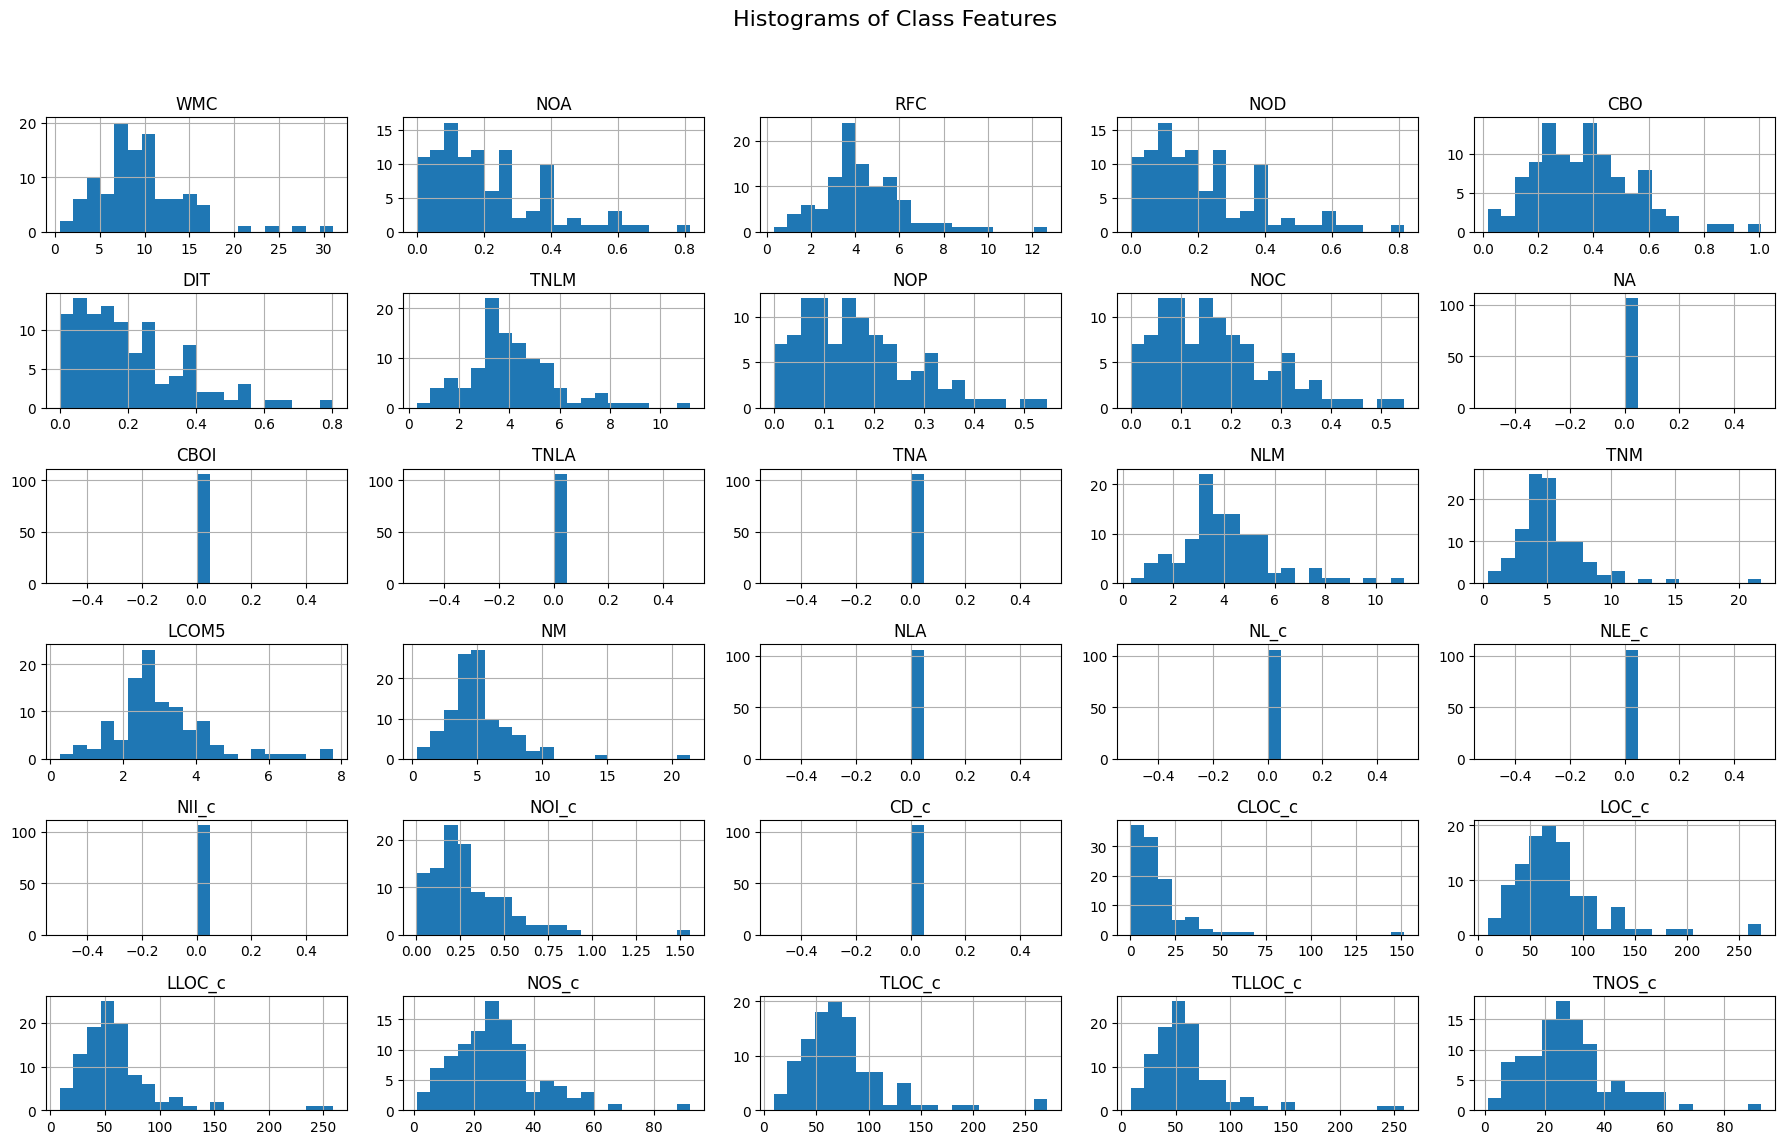
\includegraphics[height=0.95\textheight]{images/dirty-class.png}
    \caption{Histogram of Class Features (Dirty Data)}
    \label{fig:dirty-class}
\end{figure}
\end{landscape}
\restoregeometry

% Figure 2: Histogram of Class Features (Clean Data)
\begin{landscape}
\begin{figure}[!h]
    \centering
    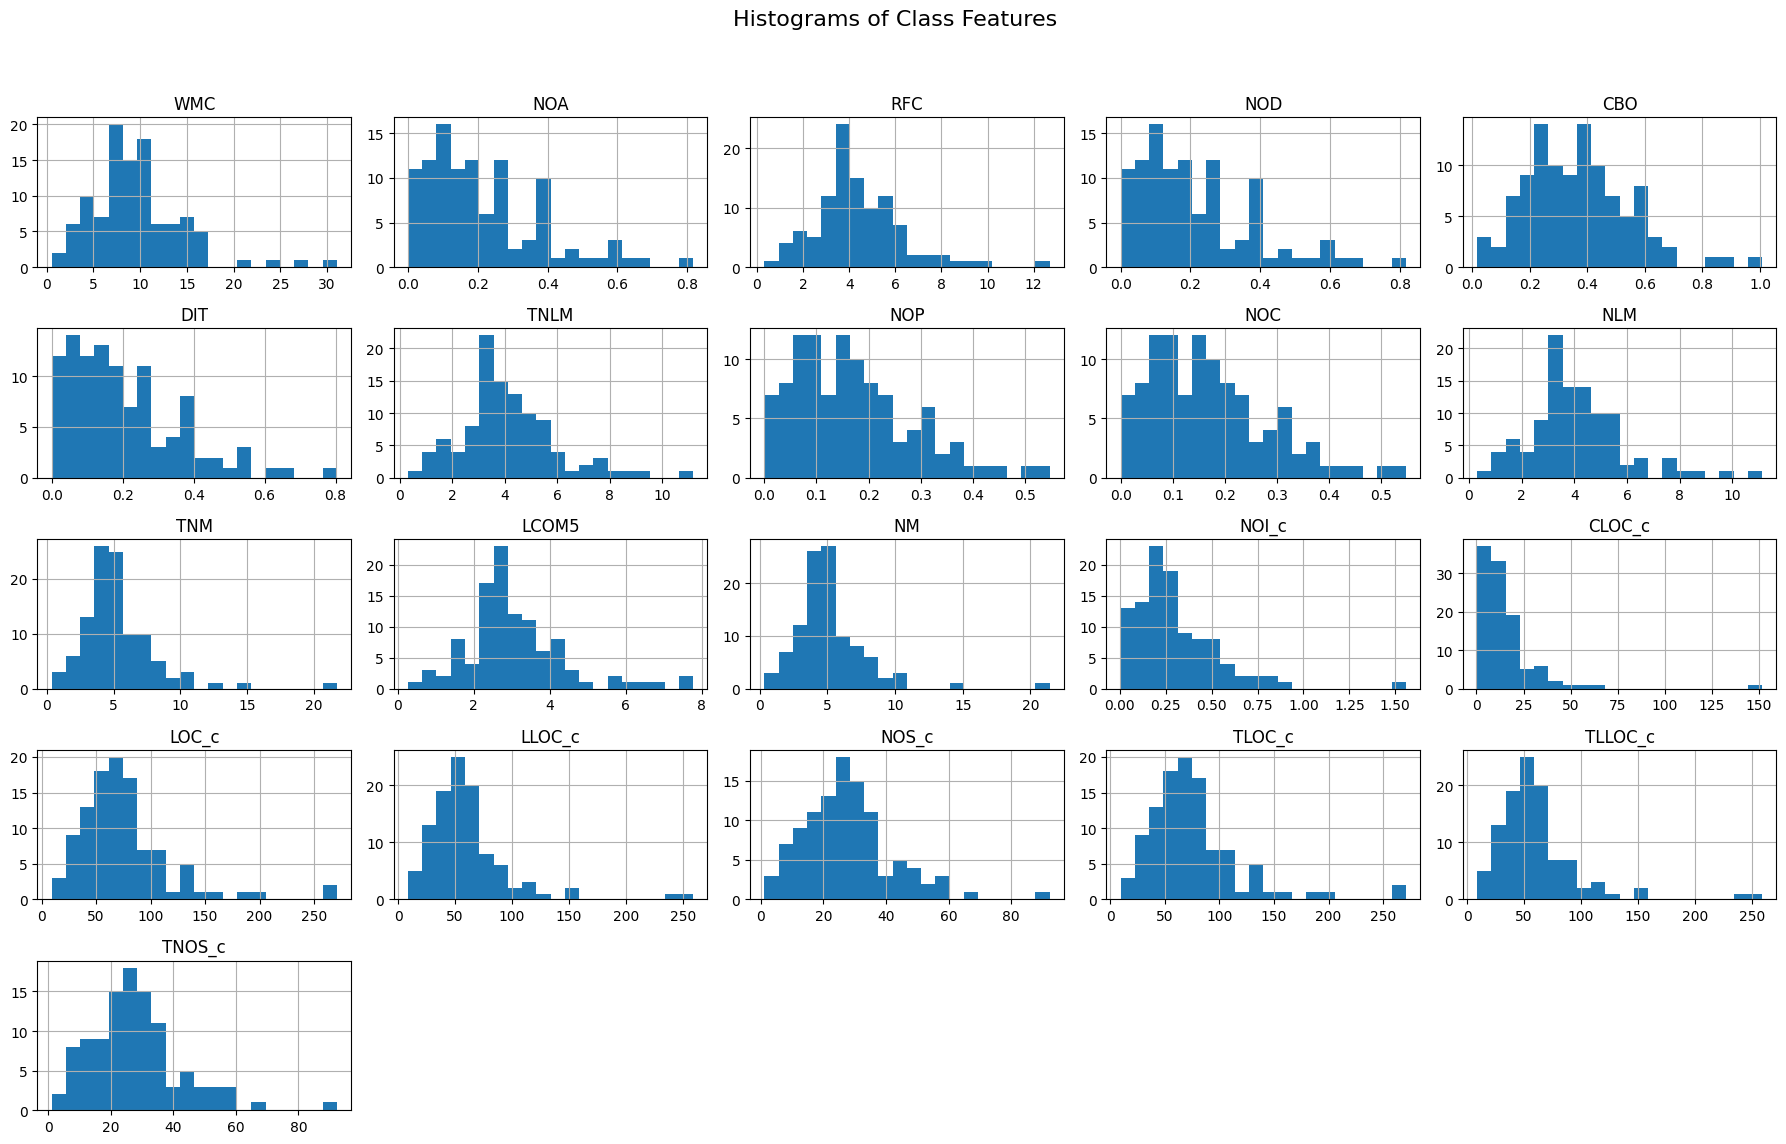
\includegraphics[height=0.95\textheight]{images/clean-class.png}
    \caption{Histogram of Class Features (Clean Data)}
    \label{fig:clean-class}
\end{figure}
\end{landscape}
\restoregeometry

% Figure 3: Histogram of Method Features (Dirty Data)
\begin{landscape}
\begin{figure}[!h]
    \centering
    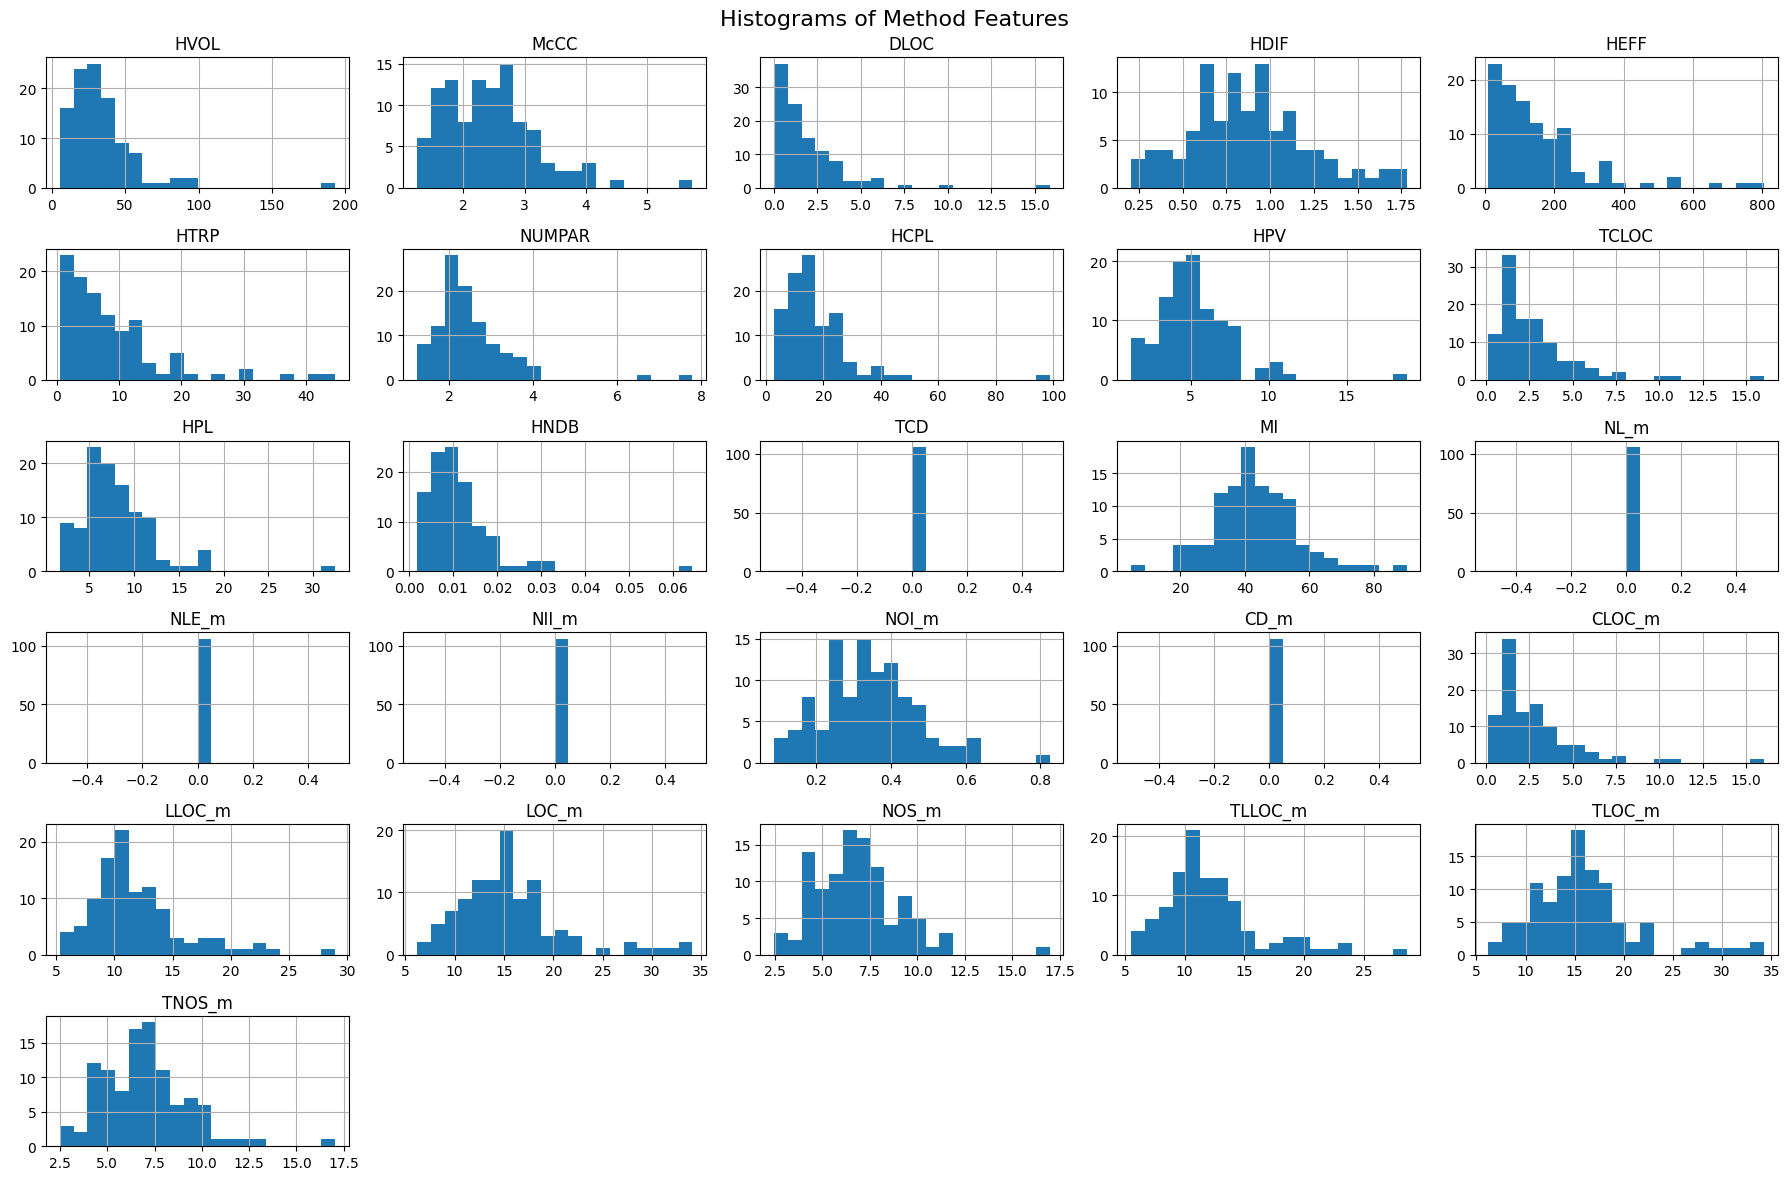
\includegraphics[height=0.95\textheight]{images/dirty-method.png}
    \caption{Histogram of Method Features (Dirty Data)}
    \label{fig:dirty-method}
\end{figure}
\end{landscape}
\restoregeometry

% Figure 4: Histogram of Method Features (Clean Data)
\begin{landscape}
\begin{figure}[!h]
    \centering
    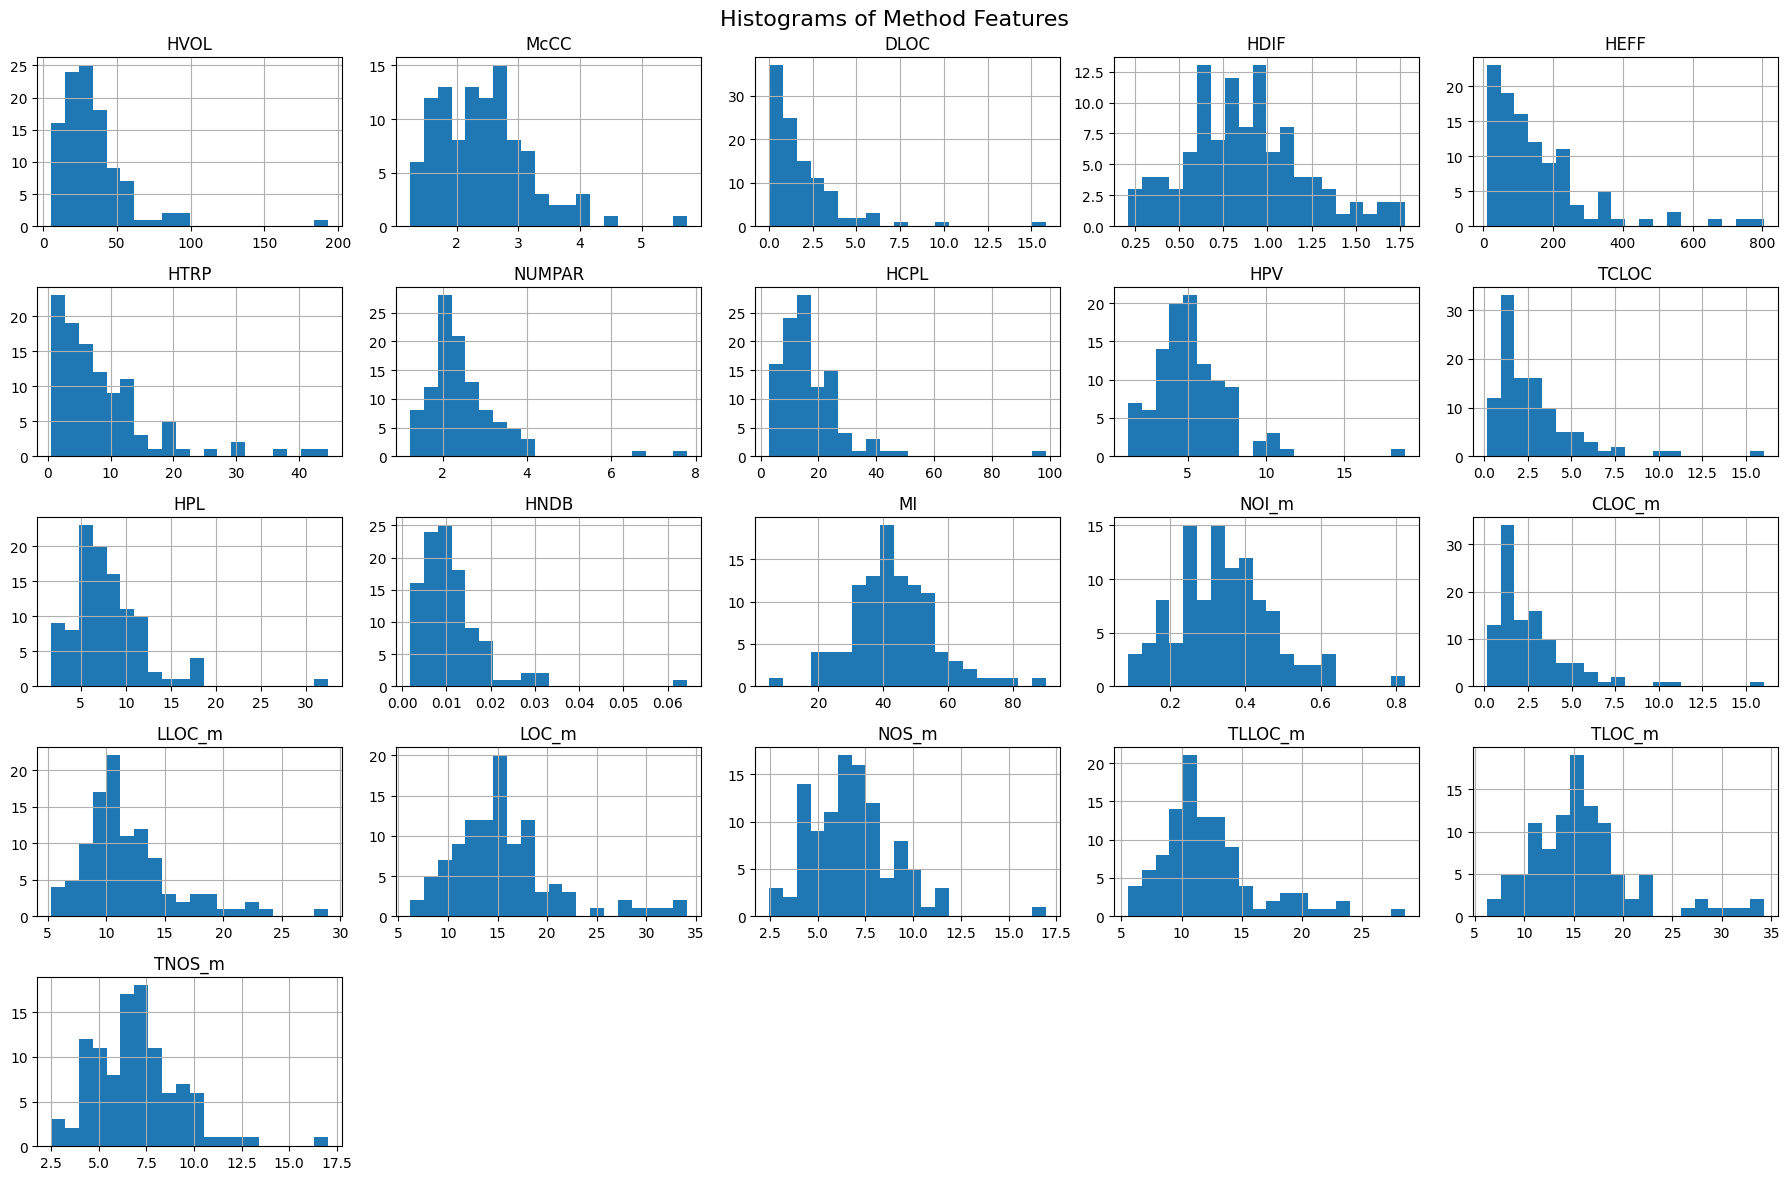
\includegraphics[height=0.95\textheight]{images/clean-method.png}
    \caption{Histogram of Method Features (Clean Data)}
    \label{fig:clean-method}
\end{figure}
\end{landscape}
\restoregeometry